\chapter{Почему Ганнибал Барка не взял Рим}

Моего любимого Ганнибала Барку постоянно упрекают в том, что он не пошел брать Рим, и поэтому слил Вторую Пунику. И это максимально дурацкая претензия к Великому Пунийцу. В которой нет вообще никакого смысла.

\section{Диспозиция}
Напоминаю диспозицию. В 218 году до нашей эры Ганнибал переходит через Альпы, прорывается в Северную Италию и в серии сражений громит римские армии одну за другой. К 216 году это заканчивается Каннами, где очередную римскую армию не просто громят, а неиллюзорно исстребляют. Это сражение имело последствия — на сторону Барки перешли Капуя и множество других южноитальянских городов. Он получил для себя ресурсную базу внутри Италии. И, казалось бы, Рим — вот он, беззащитный. Приди и возьми. Но Ганнибал на Рим не пошел, а начал обустраивать свои новые территории и вести позиционную войну с оставшимися силами Рима. Дав тому придти в себя, отмобилизоваться, и через 15 лет уже угрожать самому Карфагену. Так, по общему мнению, Барка проебал все полимеры, зассав взять Рим, когда возможность была.


Но была ли она, возможность? Щас я попробую доказать, что нет, возможности не было. И если б Ганнибал реально пошел всеми силами осаждать Рим, то проиграл бы войну не в 201г до н.э, а где-то в 215г, и запомнили бы мы его не как величайшего античного стратега, а как идиота, у которого поехала крыша от успехов, и который пошел и слился под стенами Рима безо всякого смысла.
\begin{figure}[h!tb]
	\centering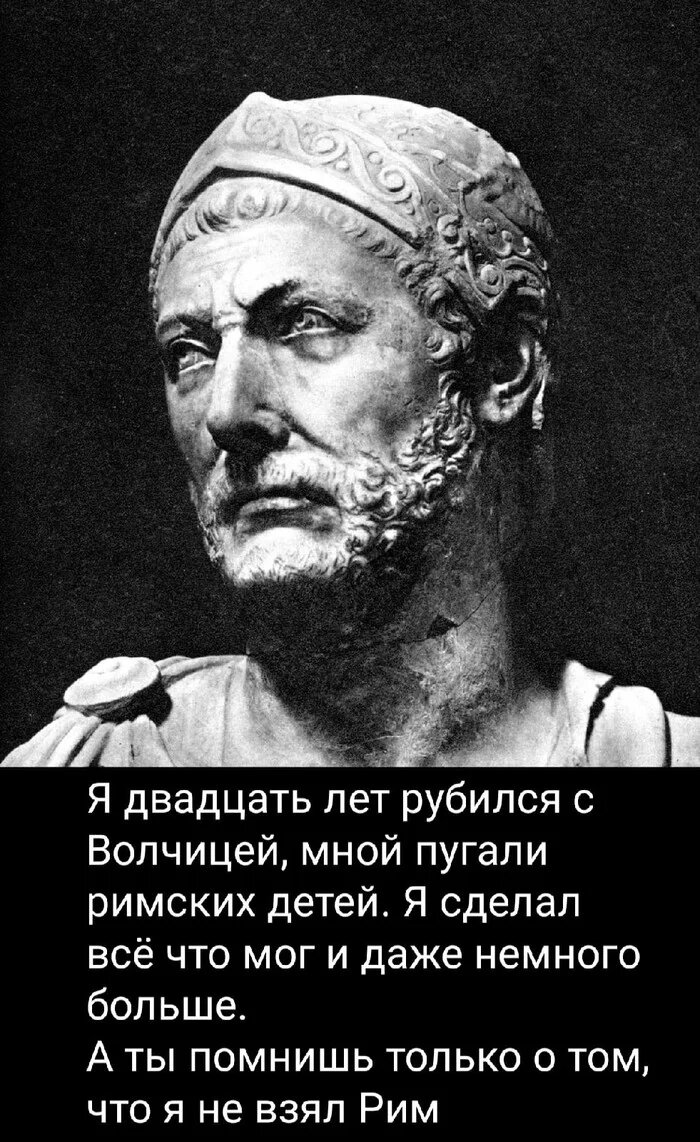
\includegraphics[scale=0.3]{Data/Hannibal_and_Rome/1622873064131436757.jpg}
	\caption{Барку огорчает современная молодежь	}
	\label{fig:barka1} % Unique label used for referencing the figure in-text
	%\addcontentsline{toc}{figure}{Figure \ref{fig:placeholder}} % Uncomment to add the figure to the table of contents
\end{figure}
\section{Рим as is}
Самое важное. Рим — это укрепленный город. Войны с этрусками и прочими самнитами были не так уж и давно. Не вчера, канешн, но тем не менее, укрепления были в порядке, а город ещë не успел разжиреть и вывалиться за свои городские стены. Предместья были, но ими бы спокойно пожертвовали. Взятие античных городов — это тот ещë гемор, осады порой длились годами и не приводили ни к чему толковому. Запас продовольствия в городе был минимум на несколько месяцев. А ещë, о чем все забывают, это большой античный латинский город. А латины, они вообще-то все военнообязанные. И хоть полевую консульскую армию Барка размотал в щепки, Рим на изи способен был выставить ополчение в несколько десятков тысяч человек, часть из которых имели боевой опыт. Да, в полевом сражении от такой армии толку мало, но на стенах она превращала штурм в практически обреченное мероприятие. А осаду Рим бы выдержал, как минимум годичную. Чет осада уже не кажется такой уж простой задачкой, не правда ли?

\begin{figure}[h!tb]
	\centering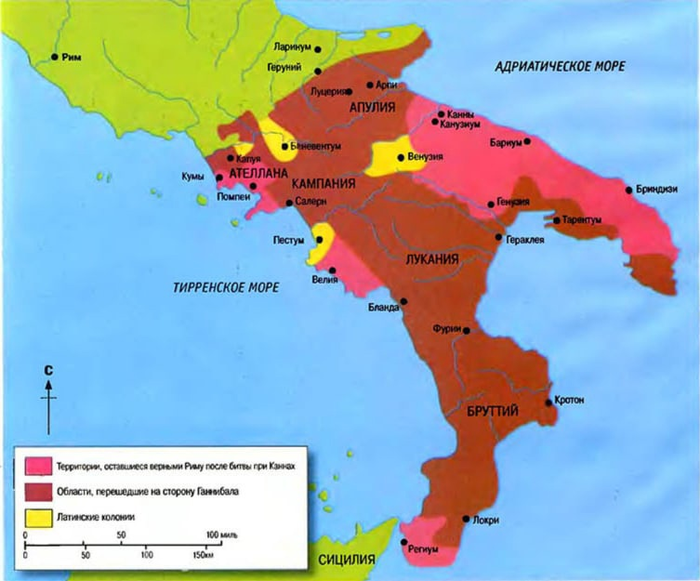
\includegraphics[scale=0.4]{Data/Hannibal_and_Rome/1622873076128424117.png}
	\caption{Вторжение или гражданка?}
	\label{fig:barka2} % Unique label used for referencing the figure in-text
	%\addcontentsline{toc}{figure}{Figure \ref{fig:placeholder}} % Uncomment to add the figure to the table of contents
\end{figure}

Идем дальше. Как я сказал выше, на сторону Барки после Канн перешли многие города Южной Италии (смотри карту). Связано это с тем, что Рим их всех не так давно завоевал, и там были довольно сильные сепаратистские настроения. Это была ресурсная база Барки, он от неë будет кормиться, снабжаться и набирать там пополнения. Именно еë наличие позволило ему продержаться так долго. Некоторые думают, что он снабжался из Африки, но это бред, так как римский флот господствовал на море, а карфагенский сенат считал эту войну авантюрой и был совершенно не рад, что баркиды еë начали. То есть для этого не было ни возможностей, ни желания. До конца войны подкрепления так и будут тягаться из Испании, сам же Карфаген так и не окажет своему лучшему полководцу никакой существенной поддержки. Поэтому лояльность южных итальянцев надо было поддерживать, находясь неподалеку и защищая их от римлян. Выдвинувшись на осаду Рима, Барка заходил в центральную Италию, где позиции Рима были очень сильны и где союзников у Пунийца не было. Не было там и снабжения. При этом Рим имел сразу два варианта действий. Можно было осадить и отрезать от снабжения самого Барку, прижав его к Городу и измотать в мелких стычках. А можно было ударить по Южной Италии и, пока Барка висит под Римом, снова подчинить себе регион. Несмотря на любовь к свободе, тамошние жители не то чтобы горели желанием вступать в тотальную войну с Римом. И поэтому точно так же, как перешли на сторону Барки после Канн, отвалились бы обратно после того, как Барка ушел бы тупить в осаде. Собственно, когда армия Пунийца эвакуировалась из Италии в Африку, так и произошло — Рим просто занял без существенного сопротивления оставленные города и занимался не столько войной, сколько террором против тех, кого считал предателями. А те даже толком не сопротивлялись. В общем, в итоге можно быть уверенным, что уйди Барка осаждать Рим, а сам Рим пообещай южноитальянцам прощение — те бы моментально предали Пунийца. Поэтому тому надо было быть рядом и держать ситуацию под контролем. И точно так же можно быть уверенным, что, потеряв Южную Италию, Барка бы не продержался против Республики и пары сезонов, несмотря на всю свою гениальность.


Выше я сказал, что штурм Баркой Рима — это из области фантастики. Да, город был большой и сильный, мог выставить мощное ополчение и беззащитным не был. Кроме того, вокруг него располагались болота, а сам он был на холмах. То есть там условия для осады максимально неудобные. Армия, особенно еë африканская часть, немедленно начнет дохнуть от климата и болезней. И даже если римляне не будут бить по коммуникациям и мешать осаде извне (а они будут), то успех абсолютно не гарантирован. Напомню, что знаменитая осада Рима галлами закончилась ничем, они простояли под стенами около года и не взяли укрепления Капитолия, после чего получили выкуп и ушли. Барка же не мог рассчитывать и на это, в первую очередь из-за состава своей армии. Которая максимально не подходила для осады и штурма городов. В основном это была легкая и средняя пехота, с достаточно низкой дисциплиной и моральным духом. Галлы и иберийцы. Также было много сильной, но бесполезной в осаде конницы. Ну и лучники с застрельщиками в ассортименте. Внимание, вопрос: кто у него там будет копать рвы, насыпать галереи, делать подкопы, строить осадные орудия и ходить на штурмы? Правильно, никто. Если римляне просто обожали осады и всегда старались что-нибудь осадить, то наемная сборная солянка Карфагена была вообще для этого неприспособлена. И гений Барки тут бы не помог. Тут никакого гения не хватит. Он отлично миксовал свою разношерстную армию и побеждал ей в полевых сражениях, но осады это совсем другое. Если в полевом сражении исход дела решается столкновением пехотных фаланг, и за несколько часов у нас уже есть победитель, в осаде в основном происходят выматывающие мелкие стычки, и которые неделя за неделей стачивают армию. Исход в них решает не гений полководца, а качество солдат и младших командиров. И нельзя сказать, что римляне по этому параметру сильно пунам уступали. В итоге осада свелась бы к позиционному размену. Чего Барка себе позволить не мог, ему неоткуда было бы снабжаться и пополняться. А вот Риму как раз этого бы и надо было. Его бы вполне устроило закидать Барку трупами, даже не в свою пользу, томушта по всей Италии подрастают маленькие латины, будущие легионеры Республики. Поэтому для Рима болезненными были только большие линейные сражения, где за несколько часов сгорали целые армии, не нанеся противнику существенных потерь. И именно ими Ганнибал с Римом и боролся, вплоть до Канн. А после, когда те отказались от генеральных сражений, Барка ими римлян пугал, постоянно вынуждая либо принимать бой, либо делать то, что ему нужно.


Подытожим.

\begin{enumerate}
	\item  Рим было не взять штурмом и было очень сложно осаждать.
	\item  Поход на Рим сразу после Канн повлек бы за собой отпадение от Карфагена Южной Италии.
	\item  Армия Барки была не приспособлена для осад.
\end{enumerate}



Чувствуете чем пахнет? Правильно, хуйней. Сама мысль о том, что надо было всë бросить и идти в лоб штурмовать Рим — максимально бредова и не выдерживает критики. Я искренне не врубаюсь кто и зачем тиражирует этот бред.

\begin{figure}[h!tb]
	\centering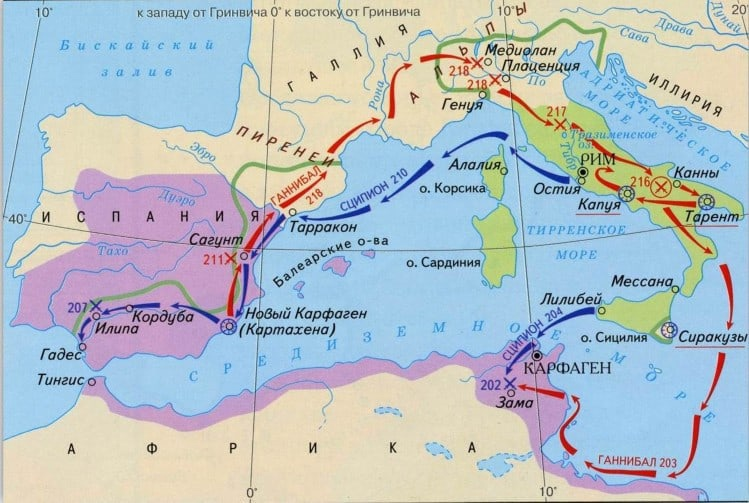
\includegraphics[scale=0.4]{Data/Hannibal_and_Rome/1622873082142334909.png}
	\caption{Долгий путь Ганнибала и не только}
	\label{fig:barka3} % Unique label used for referencing the figure in-text
	%\addcontentsline{toc}{figure}{Figure \ref{fig:placeholder}} % Uncomment to add the figure to the table of contents
\end{figure}



\section{Выводы}


Прорвавшись в Италию, Барка сломал римлянам замыслы. Они планировали в течении десятилетия двинуть на Испанию, Барка их опередил и перенес ТВД туда, где Республика не планировала воевать уже никогда. Где даже как-то и позабыли что такое война. В этом плане Ганнибал — гений. Своей серией побед он привлек на свою сторону все антиримские силы региона и мобилизовал их на борьбу. Полностью под контролем Рима оставалась только Центральная Италия, в остальных регионах союзы Рима шатались и рушились. На этом этапе Ганнибал сделал всë, что было в человеческих силах, и даже немножко больше. Он пятнадцать лет был занозой в заднице для Волчицы, и его оттуда так и не сковырнули. Сам ушел, когда Карфаген (а не Барка, обращаю внимание) все проебал на других фронтах, и римляне высадились в самой Африке. Если это не гениально, то я уже не знаю, чего вам ещë надо-то. И да, он громил римские армии везде, где у него была такая возможность, гениально используя свою рыхлую армию, собранную из говна и палок. Под его руководством этот сброд совершал чудеса на поле боя и не оставлял шансов. Он даже Заму чуть не затащил, и ему чутка не хватило до решительной победы.


Но он не взял Рим, ога. Томушта зассал, и поэтому проебал вторую Пунику. А ведь мог просто пойти и взять. Хули нам, гениям. Охуенный план, если я правильно понял. Надежный, как швейцарские часы. Я даже не знаю, как это дальше комментировать.

\section{Послесловие}

И да, войну Карфаген проиграл. Знаете почему? Томушта пока Волчица двадцать лет ебашилась с лучшим полководцем античности раз на раз, торговая республика... вообще ничего не делала. Вообще. Ничего. Вы поймите ситуацию. Баркиды — это один из влиятельнейших кланов Карфагена. Которые, после поражения в Первой Пунической, попали в опалу и позиции которых очень сильно пострадали. Де-факто в процессе Второй Пунической самим Карфагеном рулил Ганон, который был если не прямо проримским персонажем, то как минимум выступал за компромиссное решение конфликта, устраивающее всех, кроме баркидов. Последним, чтоб воевать с Римом, пришлось целую собственную страну в Испании завоевать. И все двадцать лет войны, возглавляемый Ганоном карфагенский сенат плевать хотел на Барку и его победы. И поэтому Рим победил. Томушта он воевал не с Карфагеном а именно с Баркидами, и ресурсы их были несопоставимы. И вот тут можно, да, приписать Барке его единственое в карьере неудачное решение. Возможно, ему стоило перед походом в Италию завоевать Карфаген и перерезать партию торгашей, чтоб в будущей войне с Римом иметь возможность использовать ресурсы Карфагена в полном объеме. Но это отдельная большая тема. Сегодня просто запомнили, закрепили: пока Баркиды рубились в Италии и Испании, в Африке ковыряли в носу и ничего не делали. Метрополия игнорировала просьбы о помощи от Барки и за всю войну в Италии нихера ему не дала. Более того, она сама проебала всë на свете, томушта, зачистив Испанию, римляне высадились в Африке и начали угрожать самому Карфагену. И Барка бросает свои насиженные позиции в Южной Италии, обрекая своих тамошних союзников на смерть, снимается с места, высаживается в Африке и в максимально невыгодных для себя условиях вынужден принять бой под Замой. Где он, собственно, и потерпел своë единственое поражение за всю карьеру. После чего Карфаген поднял лапки кверху и заверещал "мы сдаемся, не бейте нас, римлянушки". То есть в очередной раз повел себя максимально тупо и бесхребетно.


Ей-богу, когда через пятьдесят лет этот город сожгли к ебене матери — они все получили по заслугам. Томушта в обсуждаемые времена, походу, только Барка и понимал, что такое Рим, и какова цена этого поражения. Все остальные в торговой республике занимались чем угодно, кроме войны. А "тех, кто пали жертвой похуизма — мне ничуть не жаль".

\begin{figure}[h!tb]
	\centering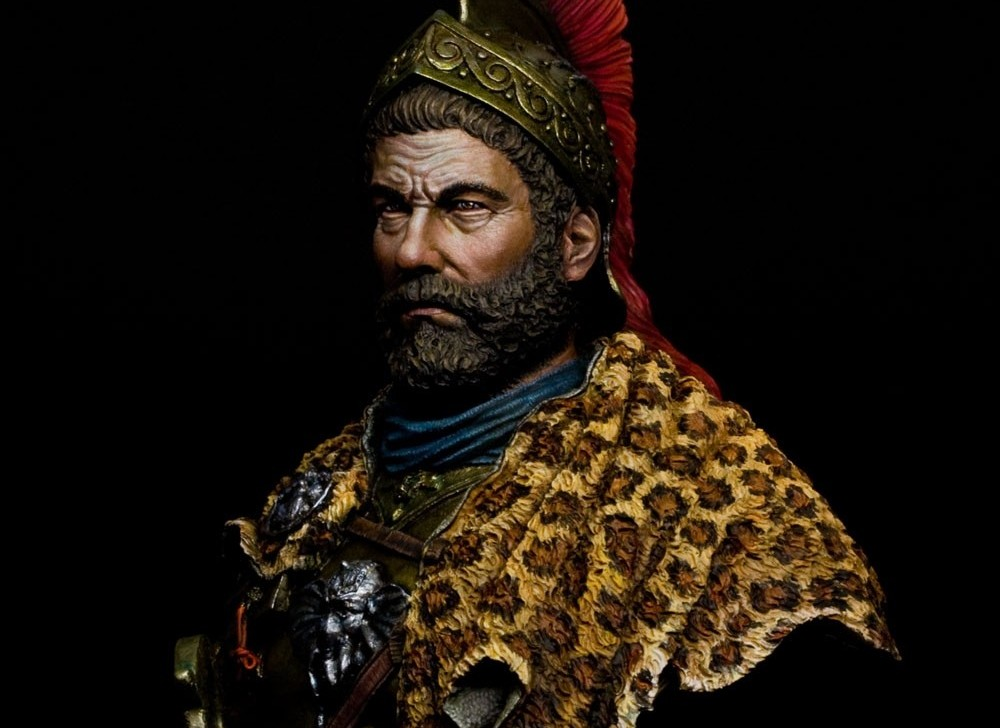
\includegraphics[scale=0.3]{Data/Hannibal_and_Rome/1622873273198376009.png}
	\caption{Барку огорчает вообще все вокруг	}
	\label{fig:barka4} % Unique label used for referencing the figure in-text
	%\addcontentsline{toc}{figure}{Figure \ref{fig:placeholder}} % Uncomment to add the figure to the table of contents
\end{figure}